\documentclass[1p]{elsarticle_modified}
%\bibliographystyle{elsarticle-num}

%\usepackage[colorlinks]{hyperref}
%\usepackage{abbrmath_seonhwa} %\Abb, \Ascr, \Acal ,\Abf, \Afrak
\usepackage{amsfonts}
\usepackage{amssymb}
\usepackage{amsmath}
\usepackage{amsthm}
\usepackage{scalefnt}
\usepackage{amsbsy}
\usepackage{kotex}
\usepackage{caption}
\usepackage{subfig}
\usepackage{color}
\usepackage{graphicx}
\usepackage{xcolor} %% white, black, red, green, blue, cyan, magenta, yellow
\usepackage{float}
\usepackage{setspace}
\usepackage{hyperref}

\usepackage{tikz}
\usetikzlibrary{arrows}

\usepackage{multirow}
\usepackage{array} % fixed length table
\usepackage{hhline}

%%%%%%%%%%%%%%%%%%%%%
\makeatletter
\renewcommand*\env@matrix[1][\arraystretch]{%
	\edef\arraystretch{#1}%
	\hskip -\arraycolsep
	\let\@ifnextchar\new@ifnextchar
	\array{*\c@MaxMatrixCols c}}
\makeatother %https://tex.stackexchange.com/questions/14071/how-can-i-increase-the-line-spacing-in-a-matrix
%%%%%%%%%%%%%%%

\usepackage[normalem]{ulem}

\newcommand{\msout}[1]{\ifmmode\text{\sout{\ensuremath{#1}}}\else\sout{#1}\fi}
%SOURCE: \msout is \stkout macro in https://tex.stackexchange.com/questions/20609/strikeout-in-math-mode

\newcommand{\cancel}[1]{
	\ifmmode
	{\color{red}\msout{#1}}
	\else
	{\color{red}\sout{#1}}
	\fi
}

\newcommand{\add}[1]{
	{\color{blue}\uwave{#1}}
}

\newcommand{\replace}[2]{
	\ifmmode
	{\color{red}\msout{#1}}{\color{blue}\uwave{#2}}
	\else
	{\color{red}\sout{#1}}{\color{blue}\uwave{#2}}
	\fi
}

\newcommand{\Sol}{\mathcal{S}} %segment
\newcommand{\D}{D} %diagram
\newcommand{\A}{\mathcal{A}} %arc


%%%%%%%%%%%%%%%%%%%%%%%%%%%%%5 test

\def\sl{\operatorname{\textup{SL}}(2,\Cbb)}
\def\psl{\operatorname{\textup{PSL}}(2,\Cbb)}
\def\quan{\mkern 1mu \triangleright \mkern 1mu}

\theoremstyle{definition}
\newtheorem{thm}{Theorem}[section]
\newtheorem{prop}[thm]{Proposition}
\newtheorem{lem}[thm]{Lemma}
\newtheorem{ques}[thm]{Question}
\newtheorem{cor}[thm]{Corollary}
\newtheorem{defn}[thm]{Definition}
\newtheorem{exam}[thm]{Example}
\newtheorem{rmk}[thm]{Remark}
\newtheorem{alg}[thm]{Algorithm}

\newcommand{\I}{\sqrt{-1}}
\begin{document}

%\begin{frontmatter}
%
%\title{Boundary parabolic representations of knots up to 8 crossings}
%
%%% Group authors per affiliation:
%\author{Yunhi Cho} 
%\address{Department of Mathematics, University of Seoul, Seoul, Korea}
%\ead{yhcho@uos.ac.kr}
%
%
%\author{Seonhwa Kim} %\fnref{s_kim}}
%\address{Center for Geometry and Physics, Institute for Basic Science, Pohang, 37673, Korea}
%\ead{ryeona17@ibs.re.kr}
%
%\author{Hyuk Kim}
%\address{Department of Mathematical Sciences, Seoul National University, Seoul 08826, Korea}
%\ead{hyukkim@snu.ac.kr}
%
%\author{Seokbeom Yoon}
%\address{Department of Mathematical Sciences, Seoul National University, Seoul, 08826,  Korea}
%\ead{sbyoon15@snu.ac.kr}
%
%\begin{abstract}
%We find all boundary parabolic representation of knots up to 8 crossings.
%
%\end{abstract}
%\begin{keyword}
%    \MSC[2010] 57M25 
%\end{keyword}
%
%\end{frontmatter}

%\linenumbers
%\tableofcontents
%
\newcommand\colored[1]{\textcolor{white}{\rule[-0.35ex]{0.8em}{1.4ex}}\kern-0.8em\color{red} #1}%
%\newcommand\colored[1]{\textcolor{white}{ #1}\kern-2.17ex	\textcolor{white}{ #1}\kern-1.81ex	\textcolor{white}{ #1}\kern-2.15ex\color{red}#1	}

{\Large $\underline{12n_{0354}~(K12n_{0354})}$}

\setlength{\tabcolsep}{10pt}
\renewcommand{\arraystretch}{1.6}
\vspace{1cm}\begin{tabular}{m{100pt}>{\centering\arraybackslash}m{274pt}}
\multirow{5}{120pt}{
	\centering
	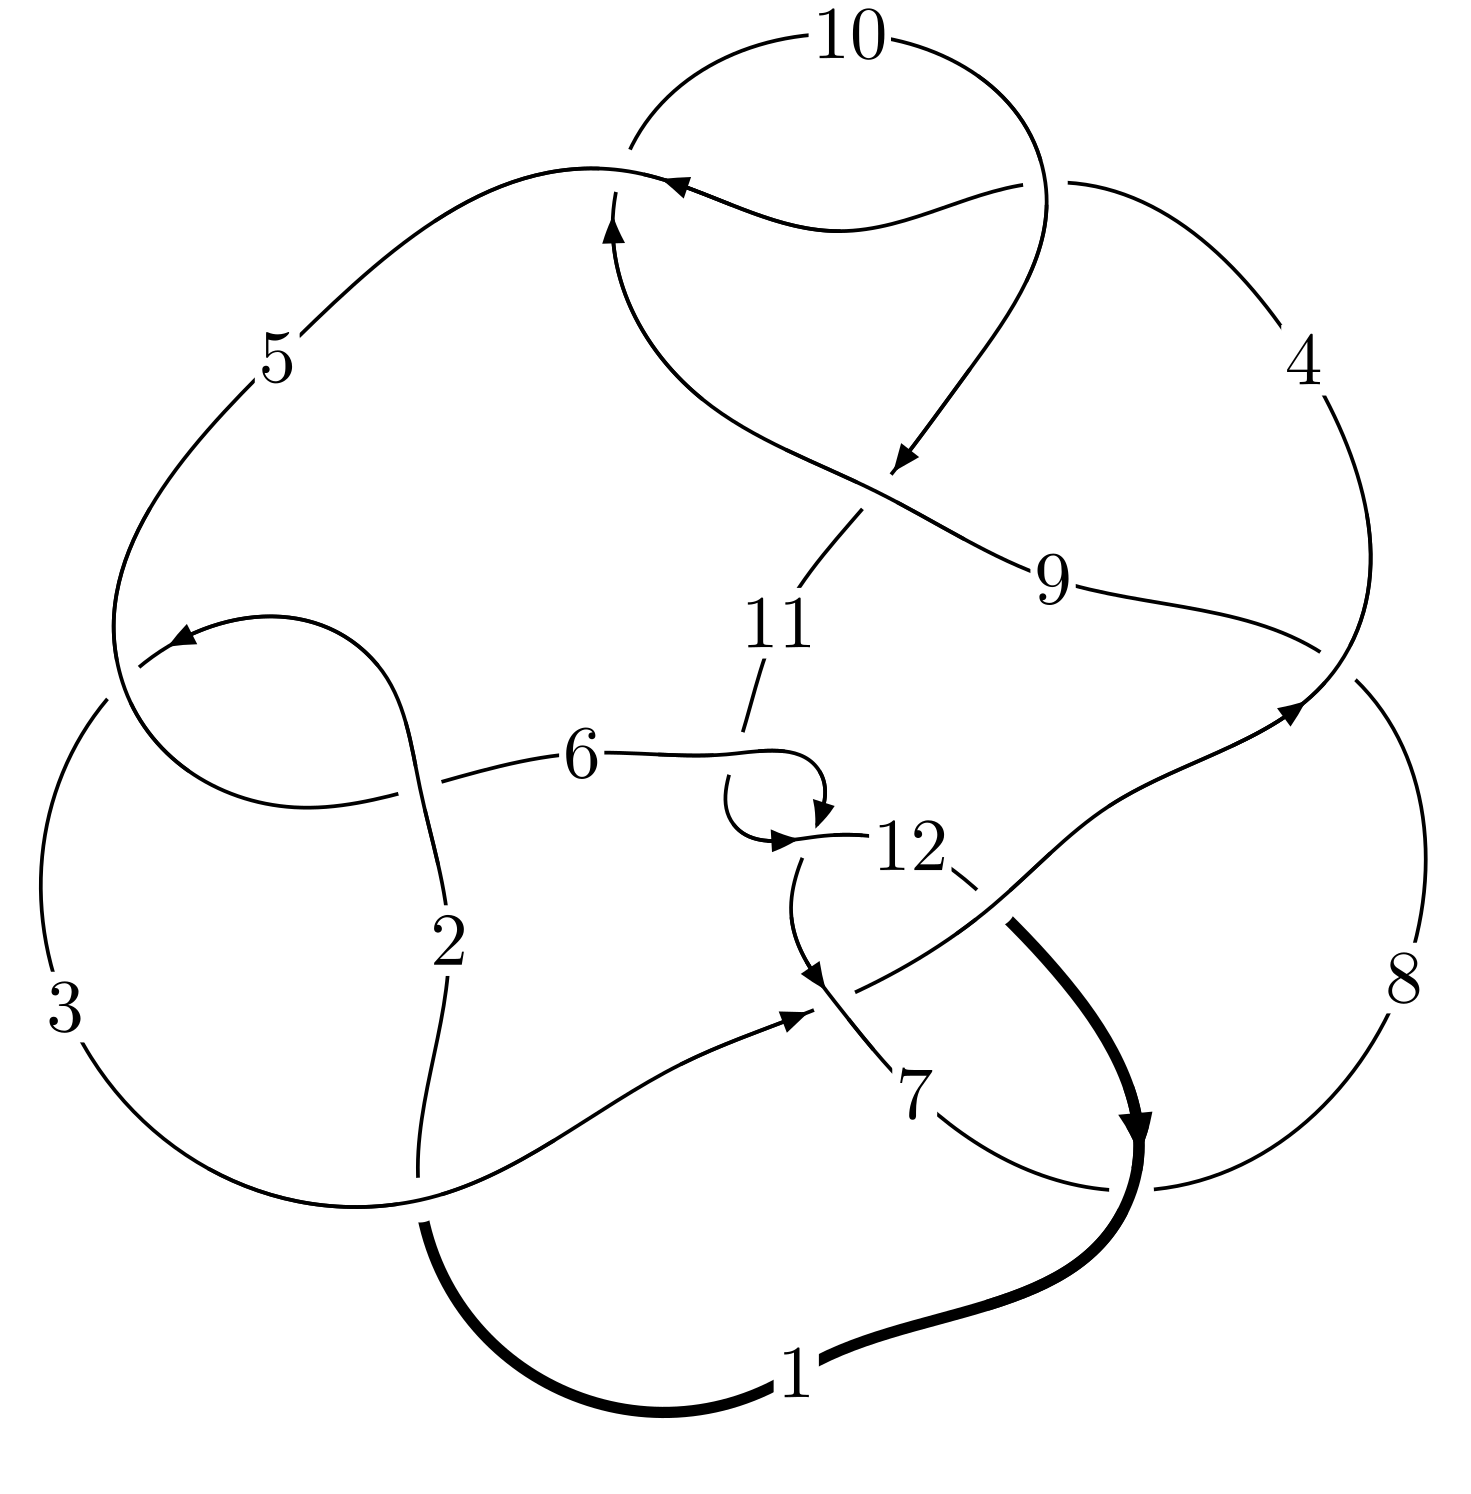
\includegraphics[width=112pt]{../../../GIT/diagram.site/Diagrams/png/2443_12n_0354.png}\\
\ \ \ A knot diagram\footnotemark}&
\allowdisplaybreaks
\textbf{Linearized knot diagam} \\
\cline{2-2}
 &
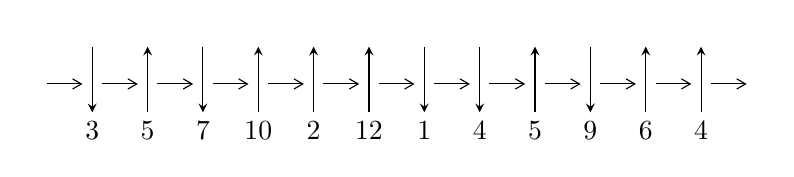
\begin{tikzpicture}[x=20pt, y=17pt]
	% nodes
	\node (C0) at (0, 0) {};
	\node (C1) at (1, 0) {};
	\node (C1U) at (1, +1) {};
	\node (C1D) at (1, -1) {3};

	\node (C2) at (2, 0) {};
	\node (C2U) at (2, +1) {};
	\node (C2D) at (2, -1) {5};

	\node (C3) at (3, 0) {};
	\node (C3U) at (3, +1) {};
	\node (C3D) at (3, -1) {7};

	\node (C4) at (4, 0) {};
	\node (C4U) at (4, +1) {};
	\node (C4D) at (4, -1) {10};

	\node (C5) at (5, 0) {};
	\node (C5U) at (5, +1) {};
	\node (C5D) at (5, -1) {2};

	\node (C6) at (6, 0) {};
	\node (C6U) at (6, +1) {};
	\node (C6D) at (6, -1) {12};

	\node (C7) at (7, 0) {};
	\node (C7U) at (7, +1) {};
	\node (C7D) at (7, -1) {1};

	\node (C8) at (8, 0) {};
	\node (C8U) at (8, +1) {};
	\node (C8D) at (8, -1) {4};

	\node (C9) at (9, 0) {};
	\node (C9U) at (9, +1) {};
	\node (C9D) at (9, -1) {5};

	\node (C10) at (10, 0) {};
	\node (C10U) at (10, +1) {};
	\node (C10D) at (10, -1) {9};

	\node (C11) at (11, 0) {};
	\node (C11U) at (11, +1) {};
	\node (C11D) at (11, -1) {6};

	\node (C12) at (12, 0) {};
	\node (C12U) at (12, +1) {};
	\node (C12D) at (12, -1) {4};
	\node (C13) at (13, 0) {};

	% arrows
	\draw[->,>={angle 60}]
	(C0) edge (C1) (C1) edge (C2) (C2) edge (C3) (C3) edge (C4) (C4) edge (C5) (C5) edge (C6) (C6) edge (C7) (C7) edge (C8) (C8) edge (C9) (C9) edge (C10) (C10) edge (C11) (C11) edge (C12) (C12) edge (C13) ;	\draw[->,>=stealth]
	(C1U) edge (C1D) (C2D) edge (C2U) (C3U) edge (C3D) (C4D) edge (C4U) (C5D) edge (C5U) (C6D) edge (C6U) (C7U) edge (C7D) (C8U) edge (C8D) (C9D) edge (C9U) (C10U) edge (C10D) (C11D) edge (C11U) (C12D) edge (C12U) ;
	\end{tikzpicture} \\
\hhline{~~} \\& 
\textbf{Solving Sequence} \\ \cline{2-2} 
 &
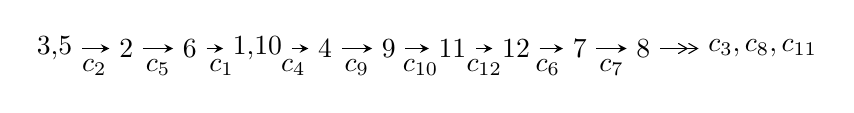
\begin{tikzpicture}[x=23pt, y=7pt]
	% node
	\node (A0) at (-1/8, 0) {3,5};
	\node (A1) at (1, 0) {2};
	\node (A2) at (2, 0) {6};
	\node (A3) at (49/16, 0) {1,10};
	\node (A4) at (33/8, 0) {4};
	\node (A5) at (41/8, 0) {9};
	\node (A6) at (49/8, 0) {11};
	\node (A7) at (57/8, 0) {12};
	\node (A8) at (65/8, 0) {7};
	\node (A9) at (73/8, 0) {8};
	\node (C1) at (1/2, -1) {$c_{2}$};
	\node (C2) at (3/2, -1) {$c_{5}$};
	\node (C3) at (5/2, -1) {$c_{1}$};
	\node (C4) at (29/8, -1) {$c_{4}$};
	\node (C5) at (37/8, -1) {$c_{9}$};
	\node (C6) at (45/8, -1) {$c_{10}$};
	\node (C7) at (53/8, -1) {$c_{12}$};
	\node (C8) at (61/8, -1) {$c_{6}$};
	\node (C9) at (69/8, -1) {$c_{7}$};
	\node (A10) at (11, 0) {$c_{3},c_{8},c_{11}$};

	% edge
	\draw[->,>=stealth]	
	(A0) edge (A1) (A1) edge (A2) (A2) edge (A3) (A3) edge (A4) (A4) edge (A5) (A5) edge (A6) (A6) edge (A7) (A7) edge (A8) (A8) edge (A9) ;
	\draw[->>,>={angle 60}]	
	(A9) edge (A10);
\end{tikzpicture} \\ 

\end{tabular} \\

\footnotetext{
The image of knot diagram is generated by the software ``\textbf{Draw programme}" developed by Andrew Bartholomew(\url{http://www.layer8.co.uk/maths/draw/index.htm\#Running-draw}), where we modified some parts for our purpose(\url{https://github.com/CATsTAILs/LinksPainter}).
}\phantom \\ \newline 
\centering \textbf{Ideals for irreducible components\footnotemark of $X_{\text{par}}$} 
 
\begin{align*}
I^u_{1}&=\langle 
-2802 u^{15}+14984 u^{14}+\cdots+11339 b+32255,\;a-1,\\
\phantom{I^u_{1}}&\phantom{= \langle  }u^{16}+4 u^{14}+16 u^{12}+u^{11}+33 u^{10}+4 u^9+45 u^8+7 u^7+38 u^6+7 u^5+21 u^4+5 u^3+7 u^2+u+1\rangle \\
I^u_{2}&=\langle 
-2 u^4- u^3+b-2 u+2,\;a+1,\;u^5+u^4+u^3+2 u^2+u+1\rangle \\
I^u_{3}&=\langle 
b-1,\;-2 u^{13}- u^{12}-6 u^{11}- u^{10}-10 u^9- u^8-10 u^7+2 u^6-7 u^5- u^4-4 u^3- u^2+a+u-1,\\
\phantom{I^u_{3}}&\phantom{= \langle  }u^{14}+4 u^{12}- u^{11}+9 u^{10}-3 u^9+13 u^8-6 u^7+14 u^6-6 u^5+11 u^4-4 u^3+5 u^2- u+1\rangle \\
I^u_{4}&=\langle 
b+1,\;-6956823038 u^{13}-6026687311 u^{12}+\cdots+24816265351 a+168071313931,\\
\phantom{I^u_{4}}&\phantom{= \langle  }u^{14}-4 u^{12}+u^{11}+15 u^{10}-3 u^9-29 u^8+8 u^7+20 u^6-14 u^5+u^4+14 u^3+11 u^2-39 u+19\rangle \\
\\
\end{align*}
\raggedright * 4 irreducible components of $\dim_{\mathbb{C}}=0$, with total 49 representations.\\
\footnotetext{All coefficients of polynomials are rational numbers. But the coefficients are sometimes approximated in decimal forms when there is not enough margin.}
\newpage
\renewcommand{\arraystretch}{1}
\centering \section*{I. $I^u_{1}= \langle -2802 u^{15}+14984 u^{14}+\cdots+11339 b+32255,\;a-1,\;u^{16}+4 u^{14}+\cdots+u+1 \rangle$}
\flushleft \textbf{(i) Arc colorings}\\
\begin{tabular}{m{7pt} m{180pt} m{7pt} m{180pt} }
\flushright $a_{3}=$&$\begin{pmatrix}1\\0\end{pmatrix}$ \\
\flushright $a_{5}=$&$\begin{pmatrix}0\\u\end{pmatrix}$ \\
\flushright $a_{2}=$&$\begin{pmatrix}1\\u^2\end{pmatrix}$ \\
\flushright $a_{6}=$&$\begin{pmatrix}u\\u^3+u\end{pmatrix}$ \\
\flushright $a_{1}=$&$\begin{pmatrix}u^2+1\\u^2\end{pmatrix}$ \\
\flushright $a_{10}=$&$\begin{pmatrix}1\\0.247112 u^{15}-1.32146 u^{14}+\cdots-4.78958 u-2.84461\end{pmatrix}$ \\
\flushright $a_{4}=$&$\begin{pmatrix}- u\\1.32146 u^{15}+0.0903960 u^{14}+\cdots+4.09172 u+0.247112\end{pmatrix}$ \\
\flushright $a_{9}=$&$\begin{pmatrix}1\\0.247112 u^{15}-1.32146 u^{14}+\cdots-4.78958 u-2.84461\end{pmatrix}$ \\
\flushright $a_{11}=$&$\begin{pmatrix}u^2+1\\0.156716 u^{15}-0.695299 u^{14}+\cdots-3.71523 u-1.52315\end{pmatrix}$ \\
\flushright $a_{12}=$&$\begin{pmatrix}-0.232560 u^{15}+0.391393 u^{14}+\cdots+0.538584 u+1.69530\\-0.0796367 u^{15}-0.619102 u^{14}+\cdots-3.33548 u-1.21924\end{pmatrix}$ \\
\flushright $a_{7}=$&$\begin{pmatrix}0.327807 u^{15}+0.339095 u^{14}+\cdots+2.63674 u-0.399859\\0.233618 u^{15}+0.650057 u^{14}+\cdots+3.55225 u+1.53021\end{pmatrix}$ \\
\flushright $a_{8}=$&$\begin{pmatrix}- u^4- u^2-1\\-0.0145515 u^{15}+0.930064 u^{14}+\cdots+4.25099 u+2.14931\end{pmatrix}$\\&\end{tabular}
\flushleft \textbf{(ii) Obstruction class $= -1$}\\~\\
\flushleft \textbf{(iii) Cusp Shapes $= \frac{20605}{11339} u^{15}+\frac{3850}{11339} u^{14}+\cdots+\frac{224602}{11339} u+\frac{37351}{11339}$}\\~\\
\newpage\renewcommand{\arraystretch}{1}
\flushleft \textbf{(iv) u-Polynomials at the component}\newline \\
\begin{tabular}{m{50pt}|m{274pt}}
Crossings & \hspace{64pt}u-Polynomials at each crossing \\
\hline $$\begin{aligned}c_{1},c_{10}\end{aligned}$$&$\begin{aligned}
&u^{16}+8 u^{15}+\cdots+13 u+1
\end{aligned}$\\
\hline $$\begin{aligned}c_{2},c_{4},c_{5}\\c_{9}\end{aligned}$$&$\begin{aligned}
&u^{16}+4 u^{14}+\cdots- u+1
\end{aligned}$\\
\hline $$\begin{aligned}c_{3}\end{aligned}$$&$\begin{aligned}
&u^{16}+5 u^{15}+\cdots+8 u+3
\end{aligned}$\\
\hline $$\begin{aligned}c_{6},c_{11},c_{12}\end{aligned}$$&$\begin{aligned}
&u^{16}+u^{15}+\cdots+2 u+1
\end{aligned}$\\
\hline $$\begin{aligned}c_{7}\end{aligned}$$&$\begin{aligned}
&u^{16}- u^{15}+\cdots+14 u+17
\end{aligned}$\\
\hline $$\begin{aligned}c_{8}\end{aligned}$$&$\begin{aligned}
&u^{16}+7 u^{14}+\cdots+13 u+5
\end{aligned}$\\
\hline
\end{tabular}\\~\\
\newpage\renewcommand{\arraystretch}{1}
\flushleft \textbf{(v) Riley Polynomials at the component}\newline \\
\begin{tabular}{m{50pt}|m{274pt}}
Crossings & \hspace{64pt}Riley Polynomials at each crossing \\
\hline $$\begin{aligned}c_{1},c_{10}\end{aligned}$$&$\begin{aligned}
&y^{16}+32 y^{15}+\cdots-7 y+1
\end{aligned}$\\
\hline $$\begin{aligned}c_{2},c_{4},c_{5}\\c_{9}\end{aligned}$$&$\begin{aligned}
&y^{16}+8 y^{15}+\cdots+13 y+1
\end{aligned}$\\
\hline $$\begin{aligned}c_{3}\end{aligned}$$&$\begin{aligned}
&y^{16}+3 y^{15}+\cdots+104 y+9
\end{aligned}$\\
\hline $$\begin{aligned}c_{6},c_{11},c_{12}\end{aligned}$$&$\begin{aligned}
&y^{16}-23 y^{15}+\cdots-22 y+1
\end{aligned}$\\
\hline $$\begin{aligned}c_{7}\end{aligned}$$&$\begin{aligned}
&y^{16}+27 y^{15}+\cdots+2796 y+289
\end{aligned}$\\
\hline $$\begin{aligned}c_{8}\end{aligned}$$&$\begin{aligned}
&y^{16}+14 y^{15}+\cdots+471 y+25
\end{aligned}$\\
\hline
\end{tabular}\\~\\
\newpage\flushleft \textbf{(vi) Complex Volumes and Cusp Shapes}
$$\begin{array}{c|c|c}  
\text{Solutions to }I^u_{1}& \I (\text{vol} + \sqrt{-1}CS) & \text{Cusp shape}\\
 \hline 
\begin{aligned}
u &= -0.530810 + 0.923327 I \\
a &= \phantom{-}1.00000\phantom{ +0.000000I} \\
b &= \phantom{-}0.789890 - 0.248067 I\end{aligned}
 & \phantom{-}2.22282 - 4.13785 I & \phantom{-}5.34445 + 5.61520 I \\ \hline\begin{aligned}
u &= -0.530810 - 0.923327 I \\
a &= \phantom{-}1.00000\phantom{ +0.000000I} \\
b &= \phantom{-}0.789890 + 0.248067 I\end{aligned}
 & \phantom{-}2.22282 + 4.13785 I & \phantom{-}5.34445 - 5.61520 I \\ \hline\begin{aligned}
u &= -0.176444 + 0.912663 I \\
a &= \phantom{-}1.00000\phantom{ +0.000000I} \\
b &= -0.297414 + 0.728074 I\end{aligned}
 & -1.53095 - 4.35219 I & -2.44817 + 6.95568 I \\ \hline\begin{aligned}
u &= -0.176444 - 0.912663 I \\
a &= \phantom{-}1.00000\phantom{ +0.000000I} \\
b &= -0.297414 - 0.728074 I\end{aligned}
 & -1.53095 + 4.35219 I & -2.44817 - 6.95568 I \\ \hline\begin{aligned}
u &= \phantom{-}0.525355 + 0.730919 I \\
a &= \phantom{-}1.00000\phantom{ +0.000000I} \\
b &= \phantom{-}1.71220 - 0.54617 I\end{aligned}
 & \phantom{-}3.44631 + 4.47005 I & \phantom{-}6.86692 - 8.13679 I \\ \hline\begin{aligned}
u &= \phantom{-}0.525355 - 0.730919 I \\
a &= \phantom{-}1.00000\phantom{ +0.000000I} \\
b &= \phantom{-}1.71220 + 0.54617 I\end{aligned}
 & \phantom{-}3.44631 - 4.47005 I & \phantom{-}6.86692 + 8.13679 I \\ \hline\begin{aligned}
u &= \phantom{-}0.462163 + 1.026620 I \\
a &= \phantom{-}1.00000\phantom{ +0.000000I} \\
b &= \phantom{-}2.11062 + 1.16455 I\end{aligned}
 & -2.50069 + 6.26666 I & -4.16993 - 5.19035 I \\ \hline\begin{aligned}
u &= \phantom{-}0.462163 - 1.026620 I \\
a &= \phantom{-}1.00000\phantom{ +0.000000I} \\
b &= \phantom{-}2.11062 - 1.16455 I\end{aligned}
 & -2.50069 - 6.26666 I & -4.16993 + 5.19035 I \\ \hline\begin{aligned}
u &= -0.370346 + 0.499709 I \\
a &= \phantom{-}1.00000\phantom{ +0.000000I} \\
b &= \phantom{-}0.423006 - 0.797373 I\end{aligned}
 & \phantom{-}0.645184 - 1.116330 I & \phantom{-}5.05748 + 5.63154 I \\ \hline\begin{aligned}
u &= -0.370346 - 0.499709 I \\
a &= \phantom{-}1.00000\phantom{ +0.000000I} \\
b &= \phantom{-}0.423006 + 0.797373 I\end{aligned}
 & \phantom{-}0.645184 + 1.116330 I & \phantom{-}5.05748 - 5.63154 I\\
 \hline 
 \end{array}$$\newpage$$\begin{array}{c|c|c}  
\text{Solutions to }I^u_{1}& \I (\text{vol} + \sqrt{-1}CS) & \text{Cusp shape}\\
 \hline 
\begin{aligned}
u &= \phantom{-}0.031146 + 0.558234 I \\
a &= \phantom{-}1.00000\phantom{ +0.000000I} \\
b &= -0.50534 - 1.74362 I\end{aligned}
 & \phantom{-}0.85013 - 1.38875 I & \phantom{-}2.96618 + 5.31348 I \\ \hline\begin{aligned}
u &= \phantom{-}0.031146 - 0.558234 I \\
a &= \phantom{-}1.00000\phantom{ +0.000000I} \\
b &= -0.50534 + 1.74362 I\end{aligned}
 & \phantom{-}0.85013 + 1.38875 I & \phantom{-}2.96618 - 5.31348 I \\ \hline\begin{aligned}
u &= -1.04563 + 1.32610 I \\
a &= \phantom{-}1.00000\phantom{ +0.000000I} \\
b &= \phantom{-}2.17161 - 0.76132 I\end{aligned}
 & \phantom{-}17.5809 - 5.0556 I & \phantom{-}3.38038 + 2.00245 I \\ \hline\begin{aligned}
u &= -1.04563 - 1.32610 I \\
a &= \phantom{-}1.00000\phantom{ +0.000000I} \\
b &= \phantom{-}2.17161 + 0.76132 I\end{aligned}
 & \phantom{-}17.5809 + 5.0556 I & \phantom{-}3.38038 - 2.00245 I \\ \hline\begin{aligned}
u &= \phantom{-}1.10456 + 1.28859 I \\
a &= \phantom{-}1.00000\phantom{ +0.000000I} \\
b &= \phantom{-}2.09543 + 0.79872 I\end{aligned}
 & \phantom{-}17.9422 + 13.0054 I & \phantom{-}3.50269 - 5.71450 I \\ \hline\begin{aligned}
u &= \phantom{-}1.10456 - 1.28859 I \\
a &= \phantom{-}1.00000\phantom{ +0.000000I} \\
b &= \phantom{-}2.09543 - 0.79872 I\end{aligned}
 & \phantom{-}17.9422 - 13.0054 I & \phantom{-}3.50269 + 5.71450 I\\
 \hline 
 \end{array}$$\newpage\newpage\renewcommand{\arraystretch}{1}
\centering \section*{II. $I^u_{2}= \langle -2 u^4- u^3+b-2 u+2,\;a+1,\;u^5+u^4+u^3+2 u^2+u+1 \rangle$}
\flushleft \textbf{(i) Arc colorings}\\
\begin{tabular}{m{7pt} m{180pt} m{7pt} m{180pt} }
\flushright $a_{3}=$&$\begin{pmatrix}1\\0\end{pmatrix}$ \\
\flushright $a_{5}=$&$\begin{pmatrix}0\\u\end{pmatrix}$ \\
\flushright $a_{2}=$&$\begin{pmatrix}1\\u^2\end{pmatrix}$ \\
\flushright $a_{6}=$&$\begin{pmatrix}u\\u^3+u\end{pmatrix}$ \\
\flushright $a_{1}=$&$\begin{pmatrix}u^2+1\\u^2\end{pmatrix}$ \\
\flushright $a_{10}=$&$\begin{pmatrix}-1\\2 u^4+u^3+2 u-2\end{pmatrix}$ \\
\flushright $a_{4}=$&$\begin{pmatrix}- u\\- u^4-2 u^3-2 u^2-3 u-2\end{pmatrix}$ \\
\flushright $a_{9}=$&$\begin{pmatrix}-1\\2 u^4+u^3- u^2+2 u-2\end{pmatrix}$ \\
\flushright $a_{11}=$&$\begin{pmatrix}- u^2-1\\-2 u^2+u-1\end{pmatrix}$ \\
\flushright $a_{12}=$&$\begin{pmatrix}0\\u^4+u\end{pmatrix}$ \\
\flushright $a_{7}=$&$\begin{pmatrix}u\\u^4+u^3+u^2+2 u\end{pmatrix}$ \\
\flushright $a_{8}=$&$\begin{pmatrix}- u^4- u^2-1\\u^4+u^3+2 u-1\end{pmatrix}$\\&\end{tabular}
\flushleft \textbf{(ii) Obstruction class $= 1$}\\~\\
\flushleft \textbf{(iii) Cusp Shapes $= 5 u^4-4 u^2$}\\~\\
\newpage\renewcommand{\arraystretch}{1}
\flushleft \textbf{(iv) u-Polynomials at the component}\newline \\
\begin{tabular}{m{50pt}|m{274pt}}
Crossings & \hspace{64pt}u-Polynomials at each crossing \\
\hline $$\begin{aligned}c_{1}\end{aligned}$$&$\begin{aligned}
&u^5- u^4- u^3+4 u^2-3 u+1
\end{aligned}$\\
\hline $$\begin{aligned}c_{2},c_{4}\end{aligned}$$&$\begin{aligned}
&u^5+u^4+u^3+2 u^2+u+1
\end{aligned}$\\
\hline $$\begin{aligned}c_{3}\end{aligned}$$&$\begin{aligned}
&u^5+4 u^4+8 u^3+9 u^2+6 u+1
\end{aligned}$\\
\hline $$\begin{aligned}c_{5},c_{9}\end{aligned}$$&$\begin{aligned}
&u^5- u^4+u^3-2 u^2+u-1
\end{aligned}$\\
\hline $$\begin{aligned}c_{6},c_{12}\end{aligned}$$&$\begin{aligned}
&u^5+2 u^4- u^3-2 u^2+1
\end{aligned}$\\
\hline $$\begin{aligned}c_{7}\end{aligned}$$&$\begin{aligned}
&u^5+2 u^4+2 u^3+3 u^2+2 u+1
\end{aligned}$\\
\hline $$\begin{aligned}c_{8}\end{aligned}$$&$\begin{aligned}
&u^5-5 u^4+6 u^3-3 u^2+u-1
\end{aligned}$\\
\hline $$\begin{aligned}c_{10}\end{aligned}$$&$\begin{aligned}
&u^5+u^4- u^3-4 u^2-3 u-1
\end{aligned}$\\
\hline $$\begin{aligned}c_{11}\end{aligned}$$&$\begin{aligned}
&u^5-2 u^4- u^3+2 u^2-1
\end{aligned}$\\
\hline
\end{tabular}\\~\\
\newpage\renewcommand{\arraystretch}{1}
\flushleft \textbf{(v) Riley Polynomials at the component}\newline \\
\begin{tabular}{m{50pt}|m{274pt}}
Crossings & \hspace{64pt}Riley Polynomials at each crossing \\
\hline $$\begin{aligned}c_{1},c_{10}\end{aligned}$$&$\begin{aligned}
&y^5-3 y^4+3 y^3-8 y^2+y-1
\end{aligned}$\\
\hline $$\begin{aligned}c_{2},c_{4},c_{5}\\c_{9}\end{aligned}$$&$\begin{aligned}
&y^5+y^4- y^3-4 y^2-3 y-1
\end{aligned}$\\
\hline $$\begin{aligned}c_{3}\end{aligned}$$&$\begin{aligned}
&y^5+4 y^3+7 y^2+18 y-1
\end{aligned}$\\
\hline $$\begin{aligned}c_{6},c_{11},c_{12}\end{aligned}$$&$\begin{aligned}
&y^5-6 y^4+9 y^3-8 y^2+4 y-1
\end{aligned}$\\
\hline $$\begin{aligned}c_{7}\end{aligned}$$&$\begin{aligned}
&y^5-4 y^3-5 y^2-2 y-1
\end{aligned}$\\
\hline $$\begin{aligned}c_{8}\end{aligned}$$&$\begin{aligned}
&y^5-13 y^4+8 y^3-7 y^2-5 y-1
\end{aligned}$\\
\hline
\end{tabular}\\~\\
\newpage\flushleft \textbf{(vi) Complex Volumes and Cusp Shapes}
$$\begin{array}{c|c|c}  
\text{Solutions to }I^u_{2}& \I (\text{vol} + \sqrt{-1}CS) & \text{Cusp shape}\\
 \hline 
\begin{aligned}
u &= \phantom{-}0.428550 + 1.039280 I \\
a &= -1.00000\phantom{ +0.000000I} \\
b &= -2.43253 - 1.66541 I\end{aligned}
 & -1.91329 + 6.77491 I & \phantom{-}3.63648 - 11.54818 I \\ \hline\begin{aligned}
u &= \phantom{-}0.428550 - 1.039280 I \\
a &= -1.00000\phantom{ +0.000000I} \\
b &= -2.43253 + 1.66541 I\end{aligned}
 & -1.91329 - 6.77491 I & \phantom{-}3.63648 + 11.54818 I \\ \hline\begin{aligned}
u &= -0.276511 + 0.728237 I \\
a &= -1.00000\phantom{ +0.000000I} \\
b &= -2.04663 + 1.96846 I\end{aligned}
 & \phantom{-}0.789751 + 0.607163 I & \phantom{-}2.03451 + 3.43880 I \\ \hline\begin{aligned}
u &= -0.276511 - 0.728237 I \\
a &= -1.00000\phantom{ +0.000000I} \\
b &= -2.04663 - 1.96846 I\end{aligned}
 & \phantom{-}0.789751 - 0.607163 I & \phantom{-}2.03451 - 3.43880 I \\ \hline\begin{aligned}
u &= -1.30408\phantom{ +0.000000I} \\
a &= -1.00000\phantom{ +0.000000I} \\
b &= -1.04169\phantom{ +0.000000I}\end{aligned}
 & \phantom{-}5.53695\phantom{ +0.000000I} & \phantom{-}7.65800\phantom{ +0.000000I}\\
 \hline 
 \end{array}$$\newpage\newpage\renewcommand{\arraystretch}{1}
\centering \section*{III. $I^u_{3}= \langle b-1,\;-2 u^{13}- u^{12}+\cdots+a-1,\;u^{14}+4 u^{12}+\cdots- u+1 \rangle$}
\flushleft \textbf{(i) Arc colorings}\\
\begin{tabular}{m{7pt} m{180pt} m{7pt} m{180pt} }
\flushright $a_{3}=$&$\begin{pmatrix}1\\0\end{pmatrix}$ \\
\flushright $a_{5}=$&$\begin{pmatrix}0\\u\end{pmatrix}$ \\
\flushright $a_{2}=$&$\begin{pmatrix}1\\u^2\end{pmatrix}$ \\
\flushright $a_{6}=$&$\begin{pmatrix}u\\u^3+u\end{pmatrix}$ \\
\flushright $a_{1}=$&$\begin{pmatrix}u^2+1\\u^2\end{pmatrix}$ \\
\flushright $a_{10}=$&$\begin{pmatrix}2 u^{13}+u^{12}+\cdots- u+1\\1\end{pmatrix}$ \\
\flushright $a_{4}=$&$\begin{pmatrix}-3 u^{13}- u^{12}+\cdots-5 u-1\\- u^{13}+2 u^{12}+\cdots-2 u+2\end{pmatrix}$ \\
\flushright $a_{9}=$&$\begin{pmatrix}2 u^{13}+u^{12}+\cdots- u+1\\-2 u^{13}- u^{12}+\cdots-2 u^2- u\end{pmatrix}$ \\
\flushright $a_{11}=$&$\begin{pmatrix}4 u^{13}+u^{12}+\cdots+6 u+2\\u^{13}+3 u^{11}+\cdots+2 u-2\end{pmatrix}$ \\
\flushright $a_{12}=$&$\begin{pmatrix}4 u^{13}+u^{12}+\cdots+6 u+3\\u^{13}+3 u^{11}+\cdots+2 u-1\end{pmatrix}$ \\
\flushright $a_{7}=$&$\begin{pmatrix}2 u^{13}-2 u^{12}+\cdots+9 u-5\\- u^{13}-3 u^{11}+u^{10}-5 u^9+2 u^8-5 u^7+3 u^6-4 u^5+u^4-2 u^3+u\end{pmatrix}$ \\
\flushright $a_{8}=$&$\begin{pmatrix}u^{13}-2 u^{12}+\cdots+5 u-4\\- u^{13}- u^{12}+\cdots+3 u-1\end{pmatrix}$\\&\end{tabular}
\flushleft \textbf{(ii) Obstruction class $= 1$}\\~\\
\flushleft \textbf{(iii) Cusp Shapes $= 3 u^{13}+5 u^{12}+13 u^{11}+17 u^{10}+25 u^9+35 u^8+30 u^7+40 u^6+19 u^5+38 u^4+10 u^3+25 u^2+14$}\\~\\
\newpage\renewcommand{\arraystretch}{1}
\flushleft \textbf{(iv) u-Polynomials at the component}\newline \\
\begin{tabular}{m{50pt}|m{274pt}}
Crossings & \hspace{64pt}u-Polynomials at each crossing \\
\hline $$\begin{aligned}c_{1}\end{aligned}$$&$\begin{aligned}
&u^{14}-8 u^{13}+\cdots-9 u+1
\end{aligned}$\\
\hline $$\begin{aligned}c_{2},c_{4}\end{aligned}$$&$\begin{aligned}
&u^{14}+4 u^{12}+\cdots- u+1
\end{aligned}$\\
\hline $$\begin{aligned}c_{3}\end{aligned}$$&$\begin{aligned}
&(u^7-2 u^6+2 u^5- u^3+2 u^2-2 u+1)^2
\end{aligned}$\\
\hline $$\begin{aligned}c_{5},c_{9}\end{aligned}$$&$\begin{aligned}
&u^{14}+4 u^{12}+\cdots+u+1
\end{aligned}$\\
\hline $$\begin{aligned}c_{6},c_{12}\end{aligned}$$&$\begin{aligned}
&u^{14}- u^{13}+\cdots+2 u+1
\end{aligned}$\\
\hline $$\begin{aligned}c_{7}\end{aligned}$$&$\begin{aligned}
&u^{14}-3 u^{13}+\cdots-2 u+1
\end{aligned}$\\
\hline $$\begin{aligned}c_{8}\end{aligned}$$&$\begin{aligned}
&u^{14}+3 u^{13}+\cdots+3 u+1
\end{aligned}$\\
\hline $$\begin{aligned}c_{10}\end{aligned}$$&$\begin{aligned}
&u^{14}+8 u^{13}+\cdots+9 u+1
\end{aligned}$\\
\hline $$\begin{aligned}c_{11}\end{aligned}$$&$\begin{aligned}
&u^{14}+u^{13}+\cdots-2 u+1
\end{aligned}$\\
\hline
\end{tabular}\\~\\
\newpage\renewcommand{\arraystretch}{1}
\flushleft \textbf{(v) Riley Polynomials at the component}\newline \\
\begin{tabular}{m{50pt}|m{274pt}}
Crossings & \hspace{64pt}Riley Polynomials at each crossing \\
\hline $$\begin{aligned}c_{1},c_{10}\end{aligned}$$&$\begin{aligned}
&y^{14}+4 y^{13}+\cdots-3 y+1
\end{aligned}$\\
\hline $$\begin{aligned}c_{2},c_{4},c_{5}\\c_{9}\end{aligned}$$&$\begin{aligned}
&y^{14}+8 y^{13}+\cdots+9 y+1
\end{aligned}$\\
\hline $$\begin{aligned}c_{3}\end{aligned}$$&$\begin{aligned}
&(y^7+2 y^5-3 y^3-1)^2
\end{aligned}$\\
\hline $$\begin{aligned}c_{6},c_{11},c_{12}\end{aligned}$$&$\begin{aligned}
&y^{14}-11 y^{13}+\cdots-6 y+1
\end{aligned}$\\
\hline $$\begin{aligned}c_{7}\end{aligned}$$&$\begin{aligned}
&y^{14}+11 y^{13}+\cdots+2 y+1
\end{aligned}$\\
\hline $$\begin{aligned}c_{8}\end{aligned}$$&$\begin{aligned}
&y^{14}+3 y^{13}+\cdots+17 y+1
\end{aligned}$\\
\hline
\end{tabular}\\~\\
\newpage\flushleft \textbf{(vi) Complex Volumes and Cusp Shapes}
$$\begin{array}{c|c|c}  
\text{Solutions to }I^u_{3}& \I (\text{vol} + \sqrt{-1}CS) & \text{Cusp shape}\\
 \hline 
\begin{aligned}
u &= \phantom{-}0.716205 + 0.619830 I \\
a &= \phantom{-}1.162750 + 0.669843 I \\
b &= \phantom{-}1.00000\phantom{ +0.000000I}\end{aligned}
 & \phantom{-}0.78568 + 5.00992 I & \phantom{-}1.33595 - 7.33845 I \\ \hline\begin{aligned}
u &= \phantom{-}0.716205 - 0.619830 I \\
a &= \phantom{-}1.162750 - 0.669843 I \\
b &= \phantom{-}1.00000\phantom{ +0.000000I}\end{aligned}
 & \phantom{-}0.78568 - 5.00992 I & \phantom{-}1.33595 + 7.33845 I \\ \hline\begin{aligned}
u &= -0.369492 + 1.060950 I \\
a &= -0.460474 + 0.495574 I \\
b &= \phantom{-}1.00000\phantom{ +0.000000I}\end{aligned}
 & -0.54326 - 3.38801 I & \phantom{-}4.33219 + 2.61481 I \\ \hline\begin{aligned}
u &= -0.369492 - 1.060950 I \\
a &= -0.460474 - 0.495574 I \\
b &= \phantom{-}1.00000\phantom{ +0.000000I}\end{aligned}
 & -0.54326 + 3.38801 I & \phantom{-}4.33219 - 2.61481 I \\ \hline\begin{aligned}
u &= -0.764704 + 0.855799 I \\
a &= \phantom{-}0.405506 - 0.437590 I \\
b &= \phantom{-}1.00000\phantom{ +0.000000I}\end{aligned}
 & \phantom{-}3.53615 - 2.90027 I & \phantom{-}8.22879 + 2.19158 I \\ \hline\begin{aligned}
u &= -0.764704 - 0.855799 I \\
a &= \phantom{-}0.405506 + 0.437590 I \\
b &= \phantom{-}1.00000\phantom{ +0.000000I}\end{aligned}
 & \phantom{-}3.53615 + 2.90027 I & \phantom{-}8.22879 - 2.19158 I \\ \hline\begin{aligned}
u &= \phantom{-}0.544331 + 1.111970 I \\
a &= \phantom{-}0.613385 + 0.789784 I \\
b &= \phantom{-}1.00000\phantom{ +0.000000I}\end{aligned}
 & -0.977413\phantom{ +0.000000I} & \phantom{-}                -6
1.206125 + 0. 10   I\phantom{ +0.000000I} \\ \hline\begin{aligned}
u &= \phantom{-}0.544331 - 1.111970 I \\
a &= \phantom{-}0.613385 - 0.789784 I \\
b &= \phantom{-}1.00000\phantom{ +0.000000I}\end{aligned}
 & -0.977413\phantom{ +0.000000I} & \phantom{-}                -6
1.206125 + 0. 10   I\phantom{ +0.000000I} \\ \hline\begin{aligned}
u &= \phantom{-}0.355639 + 0.671652 I \\
a &= -1.00622 - 1.08291 I \\
b &= \phantom{-}1.00000\phantom{ +0.000000I}\end{aligned}
 & -0.54326 - 3.38801 I & \phantom{-}4.33219 + 2.61481 I \\ \hline\begin{aligned}
u &= \phantom{-}0.355639 - 0.671652 I \\
a &= -1.00622 + 1.08291 I \\
b &= \phantom{-}1.00000\phantom{ +0.000000I}\end{aligned}
 & -0.54326 + 3.38801 I & \phantom{-}4.33219 - 2.61481 I\\
 \hline 
 \end{array}$$\newpage$$\begin{array}{c|c|c}  
\text{Solutions to }I^u_{3}& \I (\text{vol} + \sqrt{-1}CS) & \text{Cusp shape}\\
 \hline 
\begin{aligned}
u &= -0.417581 + 1.200450 I \\
a &= \phantom{-}0.645728 + 0.371994 I \\
b &= \phantom{-}1.00000\phantom{ +0.000000I}\end{aligned}
 & \phantom{-}0.78568 - 5.00992 I & \phantom{-}1.33595 + 7.33845 I \\ \hline\begin{aligned}
u &= -0.417581 - 1.200450 I \\
a &= \phantom{-}0.645728 - 0.371994 I \\
b &= \phantom{-}1.00000\phantom{ +0.000000I}\end{aligned}
 & \phantom{-}0.78568 + 5.00992 I & \phantom{-}1.33595 - 7.33845 I \\ \hline\begin{aligned}
u &= -0.064397 + 0.681658 I \\
a &= \phantom{-}1.13932 - 1.22946 I \\
b &= \phantom{-}1.00000\phantom{ +0.000000I}\end{aligned}
 & \phantom{-}3.53615 + 2.90027 I & \phantom{-}8.22879 - 2.19158 I \\ \hline\begin{aligned}
u &= -0.064397 - 0.681658 I \\
a &= \phantom{-}1.13932 + 1.22946 I \\
b &= \phantom{-}1.00000\phantom{ +0.000000I}\end{aligned}
 & \phantom{-}3.53615 - 2.90027 I & \phantom{-}8.22879 + 2.19158 I\\
 \hline 
 \end{array}$$\newpage\newpage\renewcommand{\arraystretch}{1}
\centering \section*{IV. $I^u_{4}= \langle b+1,\;-6.96\times10^{9} u^{13}-6.03\times10^{9} u^{12}+\cdots+2.48\times10^{10} a+1.68\times10^{11},\;u^{14}-4 u^{12}+\cdots-39 u+19 \rangle$}
\flushleft \textbf{(i) Arc colorings}\\
\begin{tabular}{m{7pt} m{180pt} m{7pt} m{180pt} }
\flushright $a_{3}=$&$\begin{pmatrix}1\\0\end{pmatrix}$ \\
\flushright $a_{5}=$&$\begin{pmatrix}0\\u\end{pmatrix}$ \\
\flushright $a_{2}=$&$\begin{pmatrix}1\\u^2\end{pmatrix}$ \\
\flushright $a_{6}=$&$\begin{pmatrix}u\\u^3+u\end{pmatrix}$ \\
\flushright $a_{1}=$&$\begin{pmatrix}u^2+1\\u^2\end{pmatrix}$ \\
\flushright $a_{10}=$&$\begin{pmatrix}0.280333 u^{13}+0.242852 u^{12}+\cdots+5.54317 u-6.77263\\-1\end{pmatrix}$ \\
\flushright $a_{4}=$&$\begin{pmatrix}0.478511 u^{13}+0.441369 u^{12}+\cdots+9.82537 u-9.15179\\0.242852 u^{13}+0.188871 u^{12}+\cdots+5.16037 u-5.32633\end{pmatrix}$ \\
\flushright $a_{9}=$&$\begin{pmatrix}0.280333 u^{13}+0.242852 u^{12}+\cdots+5.54317 u-6.77263\\0.188871 u^{13}+0.159671 u^{12}+\cdots+4.14491 u-5.61419\end{pmatrix}$ \\
\flushright $a_{11}=$&$\begin{pmatrix}0.763211 u^{13}+0.779348 u^{12}+\cdots+15.9697 u-14.4864\\1.00101 u^{13}+1.01426 u^{12}+\cdots+21.2588 u-20.2851\end{pmatrix}$ \\
\flushright $a_{12}=$&$\begin{pmatrix}0.258216 u^{13}+0.268552 u^{12}+\cdots+5.23924 u-4.53134\\0.00898172 u^{13}+0.00732707 u^{12}+\cdots+0.202185 u-0.624964\end{pmatrix}$ \\
\flushright $a_{7}=$&$\begin{pmatrix}0.120478 u^{13}-0.0275435 u^{12}+\cdots+3.40920 u-4.59752\\0.201962 u^{13}+0.166300 u^{12}+\cdots+4.28888 u-4.08455\end{pmatrix}$ \\
\flushright $a_{8}=$&$\begin{pmatrix}-0.945722 u^{13}-1.19104 u^{12}+\cdots-19.0444 u+13.6134\\-0.375642 u^{13}-0.447550 u^{12}+\cdots-7.86413 u+6.35879\end{pmatrix}$\\&\end{tabular}
\flushleft \textbf{(ii) Obstruction class $= -1$}\\~\\
\flushleft \textbf{(iii) Cusp Shapes $= -\frac{210581923}{1306119229} u^{13}-\frac{357801343}{1306119229} u^{12}+\cdots-\frac{6208012118}{1306119229} u+\frac{4609135372}{1306119229}$}\\~\\
\newpage\renewcommand{\arraystretch}{1}
\flushleft \textbf{(iv) u-Polynomials at the component}\newline \\
\begin{tabular}{m{50pt}|m{274pt}}
Crossings & \hspace{64pt}u-Polynomials at each crossing \\
\hline $$\begin{aligned}c_{1},c_{10}\end{aligned}$$&$\begin{aligned}
&u^{14}-8 u^{13}+\cdots-1103 u+361
\end{aligned}$\\
\hline $$\begin{aligned}c_{2},c_{4},c_{5}\\c_{9}\end{aligned}$$&$\begin{aligned}
&u^{14}-4 u^{12}+\cdots+39 u+19
\end{aligned}$\\
\hline $$\begin{aligned}c_{3}\end{aligned}$$&$\begin{aligned}
&(u^7-2 u^6+2 u^5+u^3-2 u^2+2 u-1)^2
\end{aligned}$\\
\hline $$\begin{aligned}c_{6},c_{11},c_{12}\end{aligned}$$&$\begin{aligned}
&u^{14}- u^{13}+\cdots+724 u+253
\end{aligned}$\\
\hline $$\begin{aligned}c_{7}\end{aligned}$$&$\begin{aligned}
&u^{14}-3 u^{13}+\cdots+350 u+67
\end{aligned}$\\
\hline $$\begin{aligned}c_{8}\end{aligned}$$&$\begin{aligned}
&u^{14}-3 u^{13}+\cdots-210483 u+186979
\end{aligned}$\\
\hline
\end{tabular}\\~\\
\newpage\renewcommand{\arraystretch}{1}
\flushleft \textbf{(v) Riley Polynomials at the component}\newline \\
\begin{tabular}{m{50pt}|m{274pt}}
Crossings & \hspace{64pt}Riley Polynomials at each crossing \\
\hline $$\begin{aligned}c_{1},c_{10}\end{aligned}$$&$\begin{aligned}
&y^{14}+28 y^{13}+\cdots-313387 y+130321
\end{aligned}$\\
\hline $$\begin{aligned}c_{2},c_{4},c_{5}\\c_{9}\end{aligned}$$&$\begin{aligned}
&y^{14}-8 y^{13}+\cdots-1103 y+361
\end{aligned}$\\
\hline $$\begin{aligned}c_{3}\end{aligned}$$&$\begin{aligned}
&(y^7+6 y^5+5 y^3-1)^2
\end{aligned}$\\
\hline $$\begin{aligned}c_{6},c_{11},c_{12}\end{aligned}$$&$\begin{aligned}
&y^{14}-35 y^{13}+\cdots+300098 y+64009
\end{aligned}$\\
\hline $$\begin{aligned}c_{7}\end{aligned}$$&$\begin{aligned}
&y^{14}+31 y^{13}+\cdots+16994 y+4489
\end{aligned}$\\
\hline $$\begin{aligned}c_{8}\end{aligned}$$&$\begin{aligned}
&y^{14}+103 y^{13}+\cdots-64089585027 y+34961146441
\end{aligned}$\\
\hline
\end{tabular}\\~\\
\newpage\flushleft \textbf{(vi) Complex Volumes and Cusp Shapes}
$$\begin{array}{c|c|c}  
\text{Solutions to }I^u_{4}& \I (\text{vol} + \sqrt{-1}CS) & \text{Cusp shape}\\
 \hline 
\begin{aligned}
u &= \phantom{-}0.264475 + 0.932556 I \\
a &= -0.851114 - 0.524981 I \\
b &= -1.00000\phantom{ +0.000000I}\end{aligned}
 & -3.35276\phantom{ +0.000000I} & -6.16157 + 0. I\phantom{ +0.000000I} \\ \hline\begin{aligned}
u &= \phantom{-}0.264475 - 0.932556 I \\
a &= -0.851114 + 0.524981 I \\
b &= -1.00000\phantom{ +0.000000I}\end{aligned}
 & -3.35276\phantom{ +0.000000I} & -6.16157 + 0. I\phantom{ +0.000000I} \\ \hline\begin{aligned}
u &= -0.700991 + 0.805619 I \\
a &= -0.335282 - 0.709899 I \\
b &= -1.00000\phantom{ +0.000000I}\end{aligned}
 & \phantom{-}0.20654 - 2.41511 I & \phantom{-}3.04885 + 3.06912 I \\ \hline\begin{aligned}
u &= -0.700991 - 0.805619 I \\
a &= -0.335282 + 0.709899 I \\
b &= -1.00000\phantom{ +0.000000I}\end{aligned}
 & \phantom{-}0.20654 + 2.41511 I & \phantom{-}3.04885 - 3.06912 I \\ \hline\begin{aligned}
u &= \phantom{-}1.081060 + 0.175049 I \\
a &= -1.261400 + 0.473225 I \\
b &= -1.00000\phantom{ +0.000000I}\end{aligned}
 & \phantom{-}5.81224 - 1.32363 I & \phantom{-}10.31577 + 4.85297 I \\ \hline\begin{aligned}
u &= \phantom{-}1.081060 - 0.175049 I \\
a &= -1.261400 - 0.473225 I \\
b &= -1.00000\phantom{ +0.000000I}\end{aligned}
 & \phantom{-}5.81224 + 1.32363 I & \phantom{-}10.31577 - 4.85297 I \\ \hline\begin{aligned}
u &= \phantom{-}0.806938 + 0.227524 I \\
a &= -0.543961 + 1.151740 I \\
b &= -1.00000\phantom{ +0.000000I}\end{aligned}
 & \phantom{-}0.20654 - 2.41511 I & \phantom{-}3.04885 + 3.06912 I \\ \hline\begin{aligned}
u &= \phantom{-}0.806938 - 0.227524 I \\
a &= -0.543961 - 1.151740 I \\
b &= -1.00000\phantom{ +0.000000I}\end{aligned}
 & \phantom{-}0.20654 + 2.41511 I & \phantom{-}3.04885 - 3.06912 I \\ \hline\begin{aligned}
u &= -1.44648 + 0.29078 I \\
a &= -0.694959 - 0.260721 I \\
b &= -1.00000\phantom{ +0.000000I}\end{aligned}
 & \phantom{-}5.81224 - 1.32363 I & \phantom{-}10.31577 + 4.85297 I \\ \hline\begin{aligned}
u &= -1.44648 - 0.29078 I \\
a &= -0.694959 + 0.260721 I \\
b &= -1.00000\phantom{ +0.000000I}\end{aligned}
 & \phantom{-}5.81224 + 1.32363 I & \phantom{-}10.31577 - 4.85297 I\\
 \hline 
 \end{array}$$\newpage$$\begin{array}{c|c|c}  
\text{Solutions to }I^u_{4}& \I (\text{vol} + \sqrt{-1}CS) & \text{Cusp shape}\\
 \hline 
\begin{aligned}
u &= -1.36551 + 1.07736 I \\
a &= -0.201428 - 1.007520 I \\
b &= -1.00000\phantom{ +0.000000I}\end{aligned}
 & \phantom{-}18.6867 - 3.8928 I & \phantom{-}4.21617 + 1.99955 I \\ \hline\begin{aligned}
u &= -1.36551 - 1.07736 I \\
a &= -0.201428 + 1.007520 I \\
b &= -1.00000\phantom{ +0.000000I}\end{aligned}
 & \phantom{-}18.6867 + 3.8928 I & \phantom{-}4.21617 - 1.99955 I \\ \hline\begin{aligned}
u &= \phantom{-}1.36052 + 1.15877 I \\
a &= -0.190806 + 0.954389 I \\
b &= -1.00000\phantom{ +0.000000I}\end{aligned}
 & \phantom{-}18.6867 - 3.8928 I & \phantom{-}4.21617 + 1.99955 I \\ \hline\begin{aligned}
u &= \phantom{-}1.36052 - 1.15877 I \\
a &= -0.190806 - 0.954389 I \\
b &= -1.00000\phantom{ +0.000000I}\end{aligned}
 & \phantom{-}18.6867 + 3.8928 I & \phantom{-}4.21617 - 1.99955 I\\
 \hline 
 \end{array}$$\newpage
\newpage\renewcommand{\arraystretch}{1}
\centering \section*{ V. u-Polynomials}
\begin{tabular}{m{50pt}|m{274pt}}
Crossings & \hspace{64pt}u-Polynomials at each crossing \\
\hline $$\begin{aligned}c_{1}\end{aligned}$$&$\begin{aligned}
&(u^5- u^4- u^3+4 u^2-3 u+1)(u^{14}-8 u^{13}+\cdots-9 u+1)\\
&\cdot(u^{14}-8 u^{13}+\cdots-1103 u+361)(u^{16}+8 u^{15}+\cdots+13 u+1)
\end{aligned}$\\
\hline $$\begin{aligned}c_{2},c_{4}\end{aligned}$$&$\begin{aligned}
&(u^5+u^4+u^3+2 u^2+u+1)(u^{14}-4 u^{12}+\cdots+39 u+19)\\
&\cdot(u^{14}+4 u^{12}+\cdots- u+1)(u^{16}+4 u^{14}+\cdots- u+1)
\end{aligned}$\\
\hline $$\begin{aligned}c_{3}\end{aligned}$$&$\begin{aligned}
&(u^5+4 u^4+8 u^3+9 u^2+6 u+1)(u^7-2 u^6+2 u^5- u^3+2 u^2-2 u+1)^{2}\\
&\cdot((u^7-2 u^6+2 u^5+u^3-2 u^2+2 u-1)^{2})(u^{16}+5 u^{15}+\cdots+8 u+3)
\end{aligned}$\\
\hline $$\begin{aligned}c_{5},c_{9}\end{aligned}$$&$\begin{aligned}
&(u^5- u^4+u^3-2 u^2+u-1)(u^{14}-4 u^{12}+\cdots+39 u+19)\\
&\cdot(u^{14}+4 u^{12}+\cdots+u+1)(u^{16}+4 u^{14}+\cdots- u+1)
\end{aligned}$\\
\hline $$\begin{aligned}c_{6},c_{12}\end{aligned}$$&$\begin{aligned}
&(u^5+2 u^4- u^3-2 u^2+1)(u^{14}- u^{13}+\cdots+724 u+253)\\
&\cdot(u^{14}- u^{13}+\cdots+2 u+1)(u^{16}+u^{15}+\cdots+2 u+1)
\end{aligned}$\\
\hline $$\begin{aligned}c_{7}\end{aligned}$$&$\begin{aligned}
&(u^5+2 u^4+2 u^3+3 u^2+2 u+1)(u^{14}-3 u^{13}+\cdots-2 u+1)\\
&\cdot(u^{14}-3 u^{13}+\cdots+350 u+67)(u^{16}- u^{15}+\cdots+14 u+17)
\end{aligned}$\\
\hline $$\begin{aligned}c_{8}\end{aligned}$$&$\begin{aligned}
&(u^5-5 u^4+6 u^3-3 u^2+u-1)(u^{14}-3 u^{13}+\cdots-210483 u+186979)\\
&\cdot(u^{14}+3 u^{13}+\cdots+3 u+1)(u^{16}+7 u^{14}+\cdots+13 u+5)
\end{aligned}$\\
\hline $$\begin{aligned}c_{10}\end{aligned}$$&$\begin{aligned}
&(u^5+u^4- u^3-4 u^2-3 u-1)(u^{14}-8 u^{13}+\cdots-1103 u+361)\\
&\cdot(u^{14}+8 u^{13}+\cdots+9 u+1)(u^{16}+8 u^{15}+\cdots+13 u+1)
\end{aligned}$\\
\hline $$\begin{aligned}c_{11}\end{aligned}$$&$\begin{aligned}
&(u^5-2 u^4- u^3+2 u^2-1)(u^{14}- u^{13}+\cdots+724 u+253)\\
&\cdot(u^{14}+u^{13}+\cdots-2 u+1)(u^{16}+u^{15}+\cdots+2 u+1)
\end{aligned}$\\
\hline
\end{tabular}\newpage\renewcommand{\arraystretch}{1}
\centering \section*{ VI. Riley Polynomials}
\begin{tabular}{m{50pt}|m{274pt}}
Crossings & \hspace{64pt}Riley Polynomials at each crossing \\
\hline $$\begin{aligned}c_{1},c_{10}\end{aligned}$$&$\begin{aligned}
&(y^5-3 y^4+3 y^3-8 y^2+y-1)(y^{14}+4 y^{13}+\cdots-3 y+1)\\
&\cdot(y^{14}+28 y^{13}+\cdots-313387 y+130321)(y^{16}+32 y^{15}+\cdots-7 y+1)
\end{aligned}$\\
\hline $$\begin{aligned}c_{2},c_{4},c_{5}\\c_{9}\end{aligned}$$&$\begin{aligned}
&(y^5+y^4- y^3-4 y^2-3 y-1)(y^{14}-8 y^{13}+\cdots-1103 y+361)\\
&\cdot(y^{14}+8 y^{13}+\cdots+9 y+1)(y^{16}+8 y^{15}+\cdots+13 y+1)
\end{aligned}$\\
\hline $$\begin{aligned}c_{3}\end{aligned}$$&$\begin{aligned}
&(y^5+4 y^3+\cdots+18 y-1)(y^7+2 y^5-3 y^3-1)^2(y^7+6 y^5+5 y^3-1)^2\\
&\cdot(y^{16}+3 y^{15}+\cdots+104 y+9)
\end{aligned}$\\
\hline $$\begin{aligned}c_{6},c_{11},c_{12}\end{aligned}$$&$\begin{aligned}
&(y^5-6 y^4+9 y^3-8 y^2+4 y-1)(y^{14}-35 y^{13}+\cdots+300098 y+64009)\\
&\cdot(y^{14}-11 y^{13}+\cdots-6 y+1)(y^{16}-23 y^{15}+\cdots-22 y+1)
\end{aligned}$\\
\hline $$\begin{aligned}c_{7}\end{aligned}$$&$\begin{aligned}
&(y^5-4 y^3-5 y^2-2 y-1)(y^{14}+11 y^{13}+\cdots+2 y+1)\\
&\cdot(y^{14}+31 y^{13}+\cdots+16994 y+4489)\\
&\cdot(y^{16}+27 y^{15}+\cdots+2796 y+289)
\end{aligned}$\\
\hline $$\begin{aligned}c_{8}\end{aligned}$$&$\begin{aligned}
&(y^5-13 y^4+8 y^3-7 y^2-5 y-1)(y^{14}+3 y^{13}+\cdots+17 y+1)\\
&\cdot(y^{14}+103 y^{13}+\cdots-64089585027 y+34961146441)\\
&\cdot(y^{16}+14 y^{15}+\cdots+471 y+25)
\end{aligned}$\\
\hline
\end{tabular}
\vskip 2pc
\end{document}